\documentclass[11pt]{article}
\usepackage[margin=1in]{geometry}
\usepackage{booktabs}
\usepackage{graphicx}
\usepackage{longtable}
\usepackage{array}
\usepackage{xcolor}
\usepackage{hyperref}

\title{Segmentation Evaluation Report for Magnaporthe Growth Analysis}
\author{evaluation\_report pipeline}
\date{\today}

\begin{document}
\maketitle

\section{Introduction}
This report validates a hybrid segmentation system for Magnaporthe growth analysis on ${MATCHED_PAIRS} matched annotation pairs out of ${REQUESTED_PAIRS} available predictions. The goal is to quantify how closely the final predicted segmentation contour matches the ground-truth annotation set.

\section{Methods}
\subsection{Hybrid segmentation pipeline}
${PIPELINE_DESCRIPTION}

\subsection{Evaluation protocol}
Each predicted annotation is matched to a ground-truth annotation by normalized filename stem. The polygons are rasterized into binary masks, aligned to a shared canvas when needed, and then evaluated pixel-wise. The dataset-level summary reports the mean, standard deviation, and bootstrap confidence interval of each metric.

\section{Metric definitions}
Let $TP$, $FP$, and $FN$ denote true-positive, false-positive, and false-negative pixel counts.

\[
\mathrm{Precision} = \frac{TP}{TP + FP}
\]

\[
\mathrm{Recall} = \frac{TP}{TP + FN}
\]

\[
F_1 = \frac{2 \cdot \mathrm{Precision} \cdot \mathrm{Recall}}{\mathrm{Precision} + \mathrm{Recall}}
\]

\[
\mathrm{IoU} = \frac{TP}{TP + FP + FN}
\]

\section{Results}
\subsection{Aggregate metrics}
\begin{center}
\begin{tabular}{lrrrr}
\toprule
Metric & Mean & Std & CI lower & CI upper \\
\midrule
${SUMMARY_ROWS}
\\
\bottomrule
\end{tabular}
\end{center}

\subsection{Headline values}
\begin{itemize}
\item Mean precision: ${PRECISION_MEAN}
\item Mean recall: ${RECALL_MEAN}
\item Mean F1-score: ${F1_MEAN}
\item Mean IoU: ${IOU_MEAN}
\item Missing prediction-to-GT matches: ${MISSING_PAIRS}
\end{itemize}

\subsection{Area agreement statistics}
\begin{center}
\begin{tabular}{lr}
\toprule
Statistic & Value \\
\midrule
${AREA_ROWS}
\\
\bottomrule
\end{tabular}
\end{center}

\subsection{Figures}
\begin{figure}[h!]
\centering
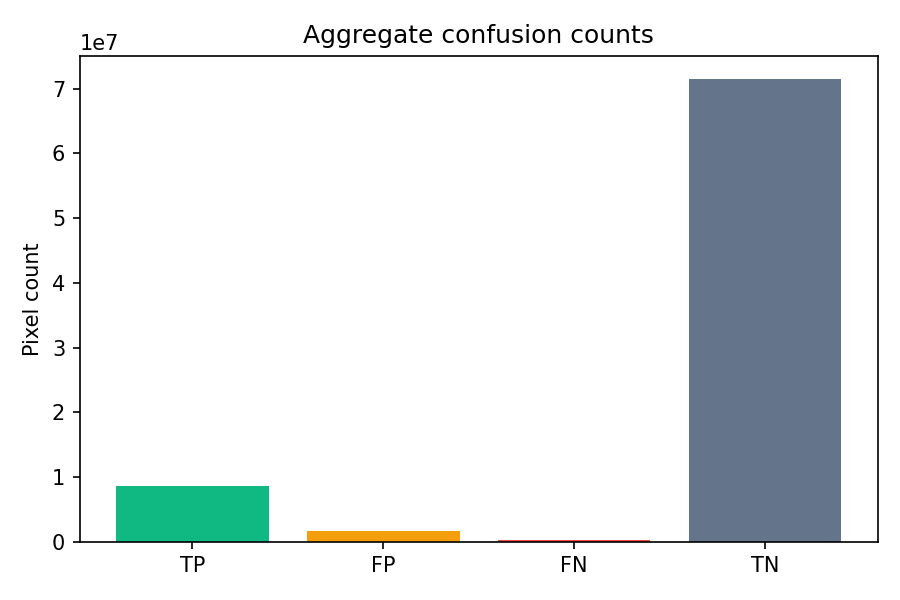
\includegraphics[width=0.7\textwidth]{figures/confusion_counts.png}
\caption{Aggregate confusion counts across the evaluation dataset.}
\end{figure}

\begin{figure}[h!]
\centering
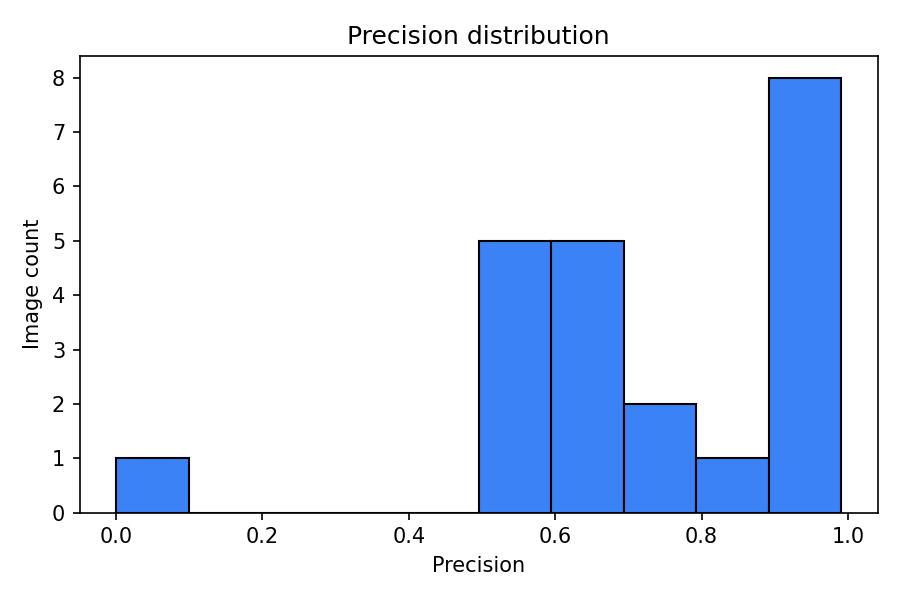
\includegraphics[width=0.48\textwidth]{figures/precision_histogram.png}
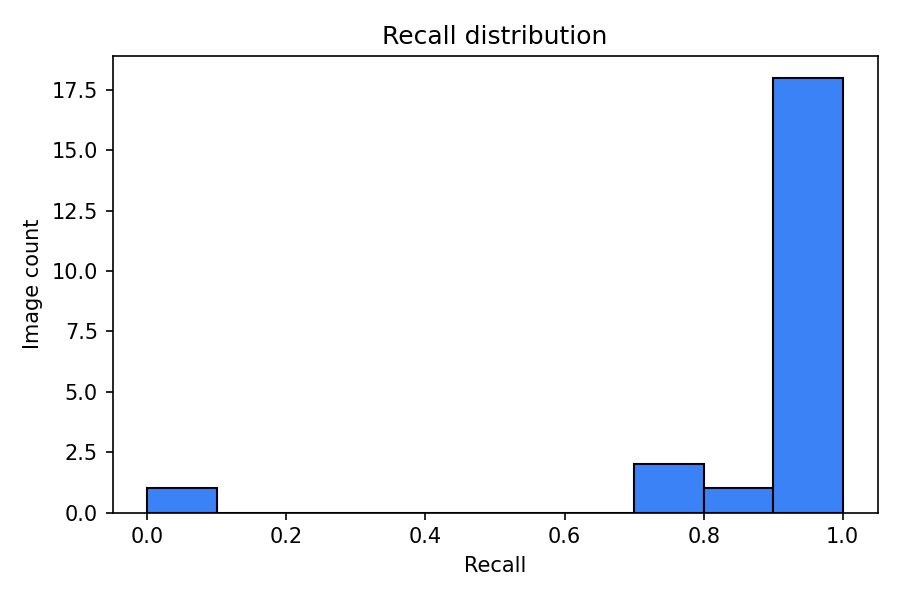
\includegraphics[width=0.48\textwidth]{figures/recall_histogram.png}
\caption{Precision and recall distributions.}
\end{figure}

\begin{figure}[h!]
\centering
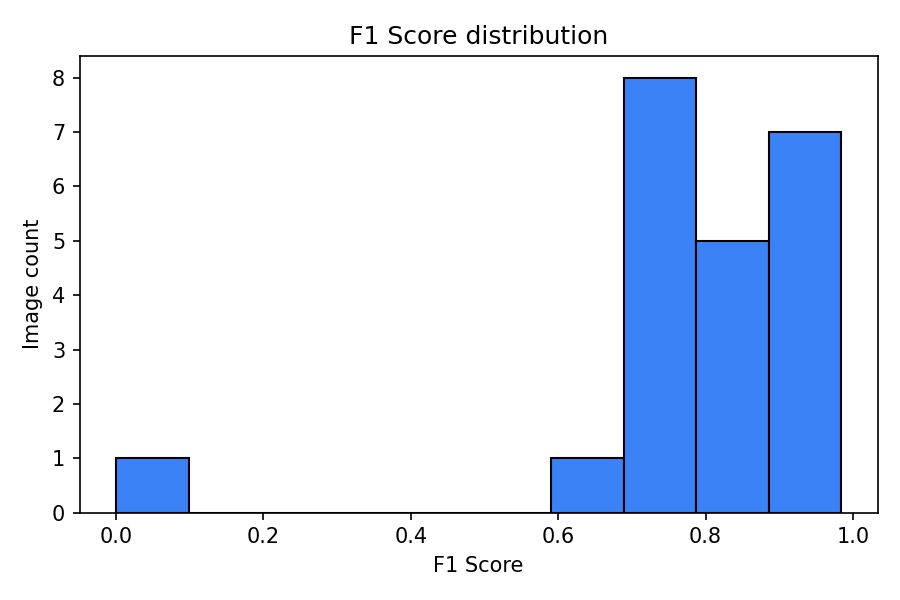
\includegraphics[width=0.48\textwidth]{figures/f1_score_histogram.png}
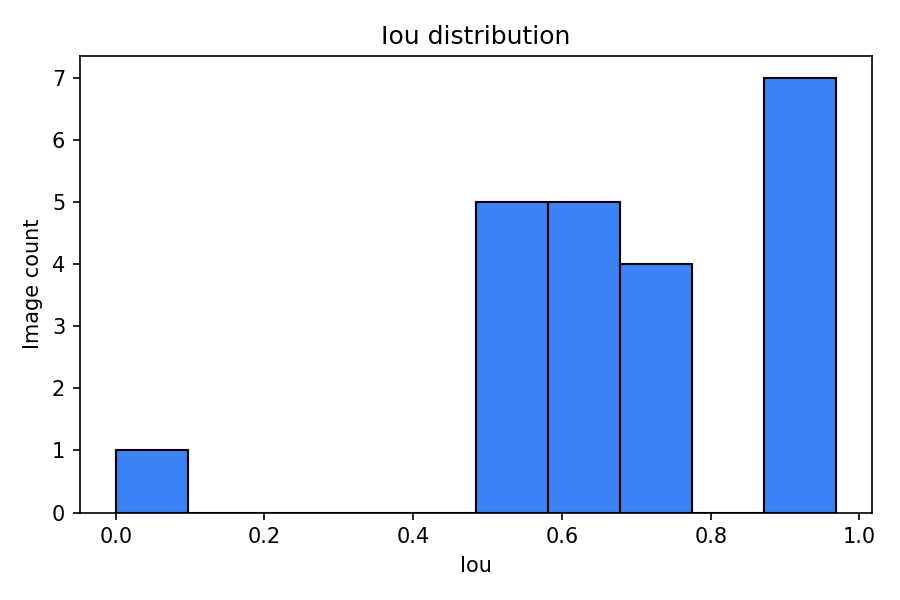
\includegraphics[width=0.48\textwidth]{figures/iou_histogram.png}
\caption{F1-score and IoU distributions.}
\end{figure}

\begin{figure}[h!]
\centering
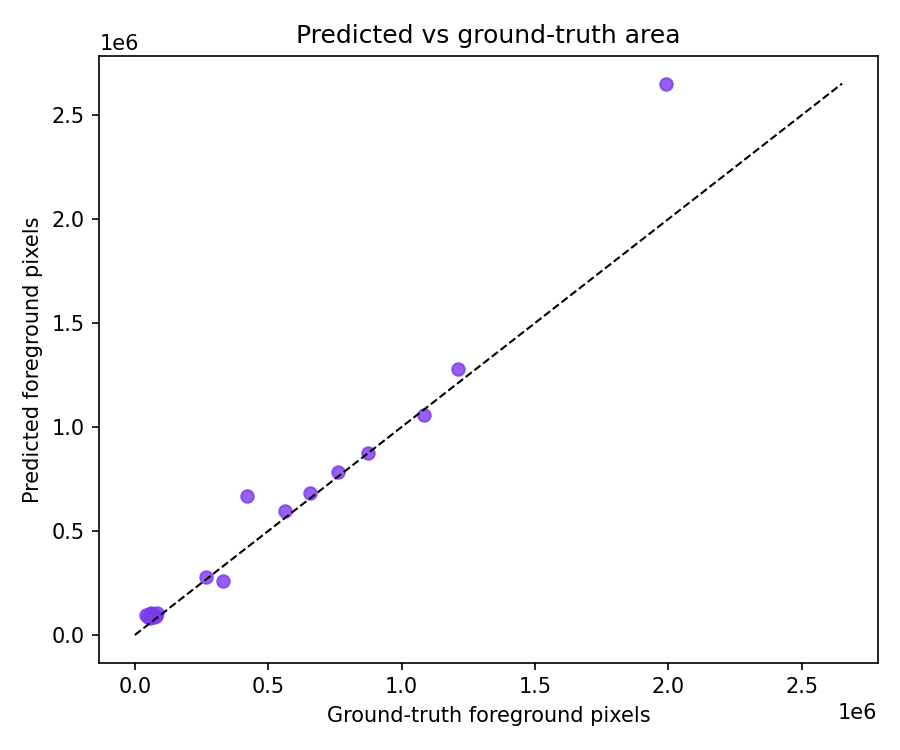
\includegraphics[width=0.48\textwidth]{figures/area_agreement.png}
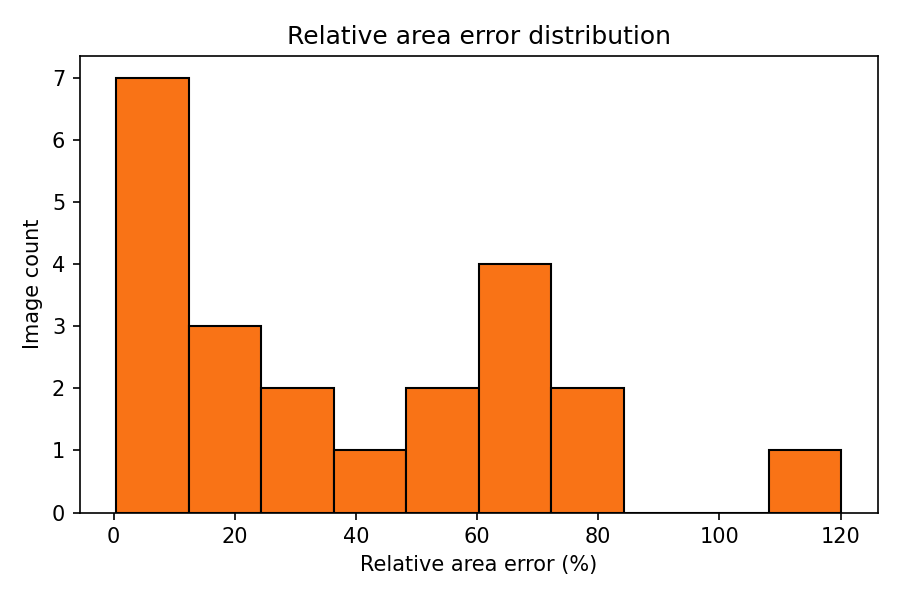
\includegraphics[width=0.48\textwidth]{figures/relative_area_error_histogram.png}
\caption{Annotation-derived area agreement and relative area error.}
\end{figure}

\section{Discussion}
The results summarize how well the final hybrid segmentation output aligns with manual ground truth on the available annotation set. Precision reflects over-segmentation control, recall reflects missed-colony risk, F1 balances both, and IoU gives a compact overlap-based score. Bootstrap confidence intervals provide a small-sample uncertainty estimate rather than a single optimistic point value.

\subsection{Conclusions}
${CONCLUSION_TEXT}

\end{document}
